\documentclass[]{book}
\usepackage{lmodern}
\usepackage{amssymb,amsmath}
\usepackage{ifxetex,ifluatex}
\usepackage{fixltx2e} % provides \textsubscript
\ifnum 0\ifxetex 1\fi\ifluatex 1\fi=0 % if pdftex
  \usepackage[T1]{fontenc}
  \usepackage[utf8]{inputenc}
\else % if luatex or xelatex
  \ifxetex
    \usepackage{mathspec}
  \else
    \usepackage{fontspec}
  \fi
  \defaultfontfeatures{Ligatures=TeX,Scale=MatchLowercase}
\fi
% use upquote if available, for straight quotes in verbatim environments
\IfFileExists{upquote.sty}{\usepackage{upquote}}{}
% use microtype if available
\IfFileExists{microtype.sty}{%
\usepackage{microtype}
\UseMicrotypeSet[protrusion]{basicmath} % disable protrusion for tt fonts
}{}
\usepackage[margin=1in]{geometry}
\usepackage{hyperref}
\hypersetup{unicode=true,
            pdftitle={Applied Time Series Analysis},
            pdfauthor={Vipul Bhatt},
            pdfborder={0 0 0},
            breaklinks=true}
\urlstyle{same}  % don't use monospace font for urls
\usepackage{natbib}
\bibliographystyle{apalike}
\usepackage{longtable,booktabs}
\usepackage{graphicx,grffile}
\makeatletter
\def\maxwidth{\ifdim\Gin@nat@width>\linewidth\linewidth\else\Gin@nat@width\fi}
\def\maxheight{\ifdim\Gin@nat@height>\textheight\textheight\else\Gin@nat@height\fi}
\makeatother
% Scale images if necessary, so that they will not overflow the page
% margins by default, and it is still possible to overwrite the defaults
% using explicit options in \includegraphics[width, height, ...]{}
\setkeys{Gin}{width=\maxwidth,height=\maxheight,keepaspectratio}
\IfFileExists{parskip.sty}{%
\usepackage{parskip}
}{% else
\setlength{\parindent}{0pt}
\setlength{\parskip}{6pt plus 2pt minus 1pt}
}
\setlength{\emergencystretch}{3em}  % prevent overfull lines
\providecommand{\tightlist}{%
  \setlength{\itemsep}{0pt}\setlength{\parskip}{0pt}}
\setcounter{secnumdepth}{5}
% Redefines (sub)paragraphs to behave more like sections
\ifx\paragraph\undefined\else
\let\oldparagraph\paragraph
\renewcommand{\paragraph}[1]{\oldparagraph{#1}\mbox{}}
\fi
\ifx\subparagraph\undefined\else
\let\oldsubparagraph\subparagraph
\renewcommand{\subparagraph}[1]{\oldsubparagraph{#1}\mbox{}}
\fi

%%% Use protect on footnotes to avoid problems with footnotes in titles
\let\rmarkdownfootnote\footnote%
\def\footnote{\protect\rmarkdownfootnote}

%%% Change title format to be more compact
\usepackage{titling}

% Create subtitle command for use in maketitle
\newcommand{\subtitle}[1]{
  \posttitle{
    \begin{center}\large#1\end{center}
    }
}

\setlength{\droptitle}{-2em}

  \title{Applied Time Series Analysis}
    \pretitle{\vspace{\droptitle}\centering\huge}
  \posttitle{\par}
    \author{Vipul Bhatt}
    \preauthor{\centering\large\emph}
  \postauthor{\par}
      \predate{\centering\large\emph}
  \postdate{\par}
    \date{2018-07-31}

\usepackage{booktabs}
\usepackage{amsthm}
\makeatletter
\def\thm@space@setup{%
  \thm@preskip=8pt plus 2pt minus 4pt
  \thm@postskip=\thm@preskip
}
\makeatother

\usepackage{amsthm}
\newtheorem{theorem}{Theorem}[chapter]
\newtheorem{lemma}{Lemma}[chapter]
\theoremstyle{definition}
\newtheorem{definition}{Definition}[chapter]
\newtheorem{corollary}{Corollary}[chapter]
\newtheorem{proposition}{Proposition}[chapter]
\theoremstyle{definition}
\newtheorem{example}{Example}[chapter]
\theoremstyle{definition}
\newtheorem{exercise}{Exercise}[chapter]
\theoremstyle{remark}
\newtheorem*{remark}{Remark}
\newtheorem*{solution}{Solution}
\let\BeginKnitrBlock\begin \let\EndKnitrBlock\end
\begin{document}
\maketitle

{
\setcounter{tocdepth}{1}
\tableofcontents
}
\chapter*{Preface}\label{preface}
\addcontentsline{toc}{chapter}{Preface}

These lecture notes are prepared for an upper level undergraduate course
in time series econometrics. Every fall I teach a course on applied time
series analysis at James Madison University. These notes borrow heavliy
from the teaching material that I have developed over several years of
instruction of this course.

One of my main objective is to develop a primer on time series analysis
that is more accessible to undergraduate students than standard
textbooks available in the market. Most of these textbooks in my opinion
are densely written and assume advanced mathematical skills on the part
of our students. Further, I have also struggled with their topic
selection and organization. Often I end up not following the chapters in
order and modify content (by adding or subtracting) to meet my students
needs. Such changes causes confusion for some students and more
importantly discourages optimal use of the textbook. Hence, this is an
undertaking to develop a primer on time series that is accessible,
follows a more logical sequencing of topics, and covers content that is
most useful for undergraduate students in business and economics.

\emph{Note: These notes have been prepared by me using various sources,
published and unpublished. All errors that remain are mine.}

\chapter{Introduction to Forecasting}\label{intro}

\section{Time Series}\label{time-series}

A time series is a specific kind of data where observations of a
variable are recorded over time. For example, the data for the U.S. GDP
for the last 30 years is a time series data.

Such data shows how a variable is changing over time. Depending on the
variable of interest we can have data measured at different frequencies.
Some commonly used frequencies are intra-day, daily, weekly, monthly,
quarterly, semi-annual and annual. Figure \ref{fig:figone} below plots
data for quarterly and monthly frequency.

\begin{figure}

{\centering 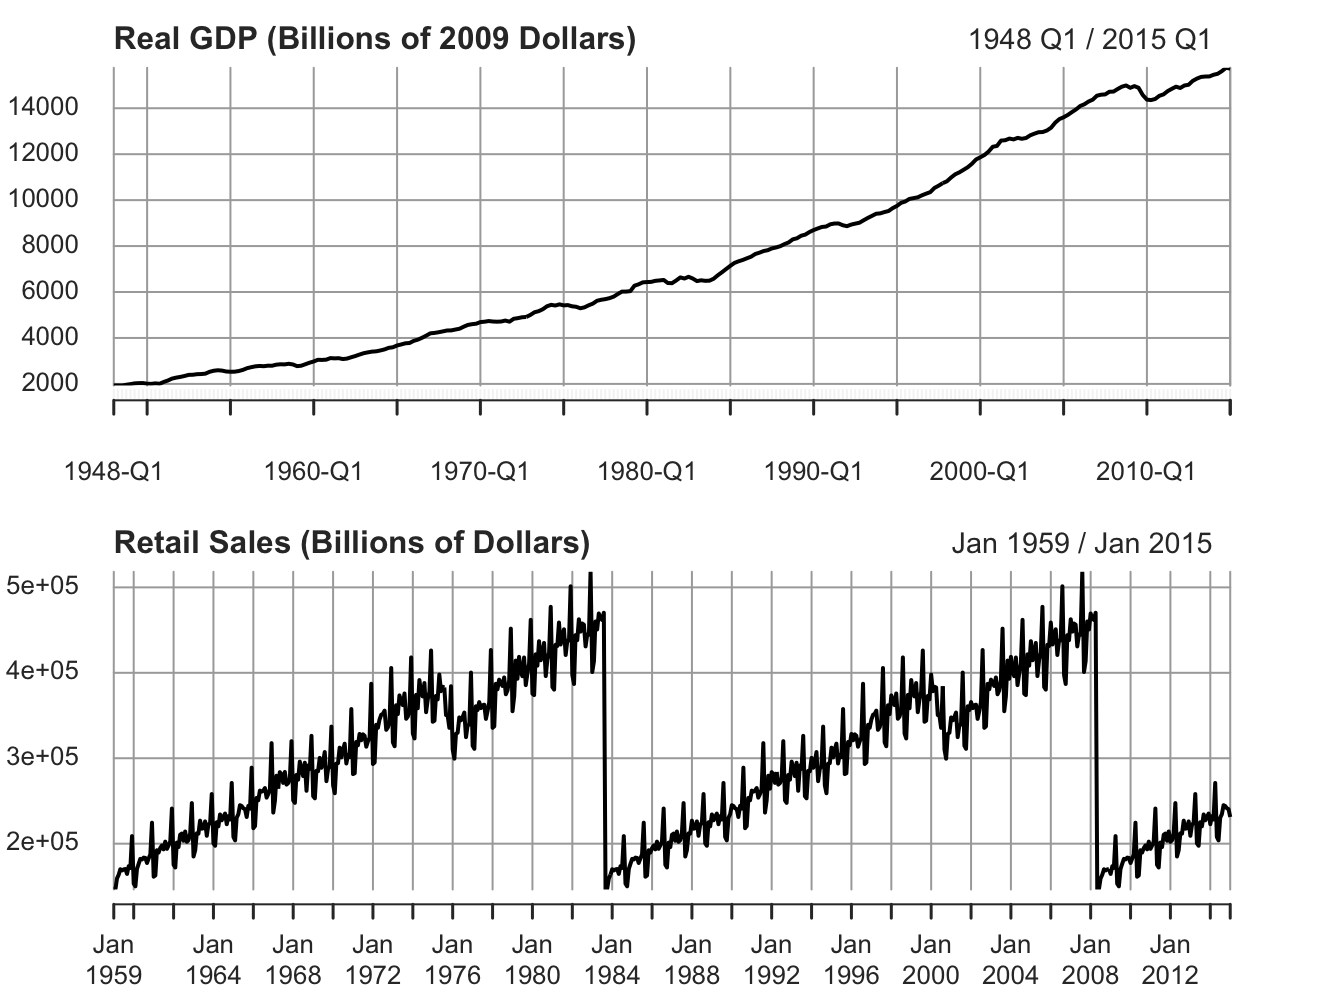
\includegraphics[width=0.8\linewidth]{bookdown-demo_files/figure-latex/figone-1} 

}

\caption{Time Series at quarterly and monthly frequency}\label{fig:figone}
\end{figure}

The first panel shows data for the real gross domestic product (GDP) for
the US in 2009 dollars, measured at a quarterly frequency. The second
panel shows data for the retail sales in the U.S. billions of dollars,
measured at monthly frequency.

Formally, we denote a time series variable by \(y_t\), where
\(t=0,1,2,..,T\) is the observation index. For example, at \(t=10\) we
get the tenth observation of this time series, \(y_{10}\).

\subsection{Serial Correlation}\label{serial-correlation}

Serial correlation is a measure of temporal dynamics of a time series.
It addresses the following question: what is the effect of past
realizations of a time series on the current period value? Formally,

\begin{equation}
\rho(s)=Cor(y_t, y_{t-s}) =\frac{   Cov(y_t,y_{t-s})}{\sqrt{\sigma^2_{y_t} \times \sigma^2_{y_{t-s}}}}
\end{equation}

where \(Cov(y_t,y_{t-s})= E(y_t-\mu_{y_t})(y_{t-s}-\mu_{y_{t-s}})\) and
\(\sigma^2_{y_t}=E(y_t-\mu_{y_t})^2\)

Here, \(\rho(s)\) is the serial correlation of order \(s\). Note that
often we use historical data to forecast. If there is no serial
correlation, then past can offer no guidance for the present and future.
In that sense, presence of serial correlation of some order is the first
condition for being able to forecast a time series using its historical
realizations.

\subsection{White Noise Process}\label{white-noise-process}

A time series is a \emph{white noise} process is it has zero mean,
constant and finite variance, and is seriall uncorrelated. Formally,
\(y_t\) is a white noise process if:

\begin{enumerate}
\def\labelenumi{\arabic{enumi}.}
\tightlist
\item
  \(E(y_t)=0\)
\item
  \(Var(y_t)=\sigma^2_y\)
\item
  \(Cov(y_t,y_{t-s})= 0 \forall s\neq t\)
\end{enumerate}

We can compress the above definition as: \(y_t\sim WN(0,\sigma^2_y)\).
Often we assume that the unexplained part of a time series follows a
white noise process. By definition we cannot forecast a white noise
process. An important diagnostics of model adequacy is to test whether
the estimated residuals are white noise (more on this later).

\section{Important Elements of
Forecasting}\label{important-elements-of-forecasting}

\BeginKnitrBlock{definition}[Forecast]
\protect\hypertarget{def:d1}{}{\label{def:d1} \iffalse (Forecast) \fi{} }
\EndKnitrBlock{definition} A \emph{forecast} is an \emph{informed} guess
about the unknow future value of a time series of interest. For example,
what is the stock price of Facebook next Monday?

There are three possible types of forecasts:

\begin{enumerate}
\def\labelenumi{\arabic{enumi}.}
\tightlist
\item
  \emph{Density Forecast}: we forecast the entire probability
  distribution of the possible future value of the time series of
  interest. Hence,
\end{enumerate}

\begin{equation}
F(a)=P[y_{t+1}\leq a]
\end{equation}

give us the probability that the 1-period ahead future value of
\(y_{t+1}\) will be less than or equal to \(a\). For example, the future
real GDP growth could be normally distributed with a mean of 1.3\% and a
standard deviation of 1.83\%. Figure \ref{fig:figtwo} below plots the
density forecast for real GDP growth.

\begin{figure}

{\centering 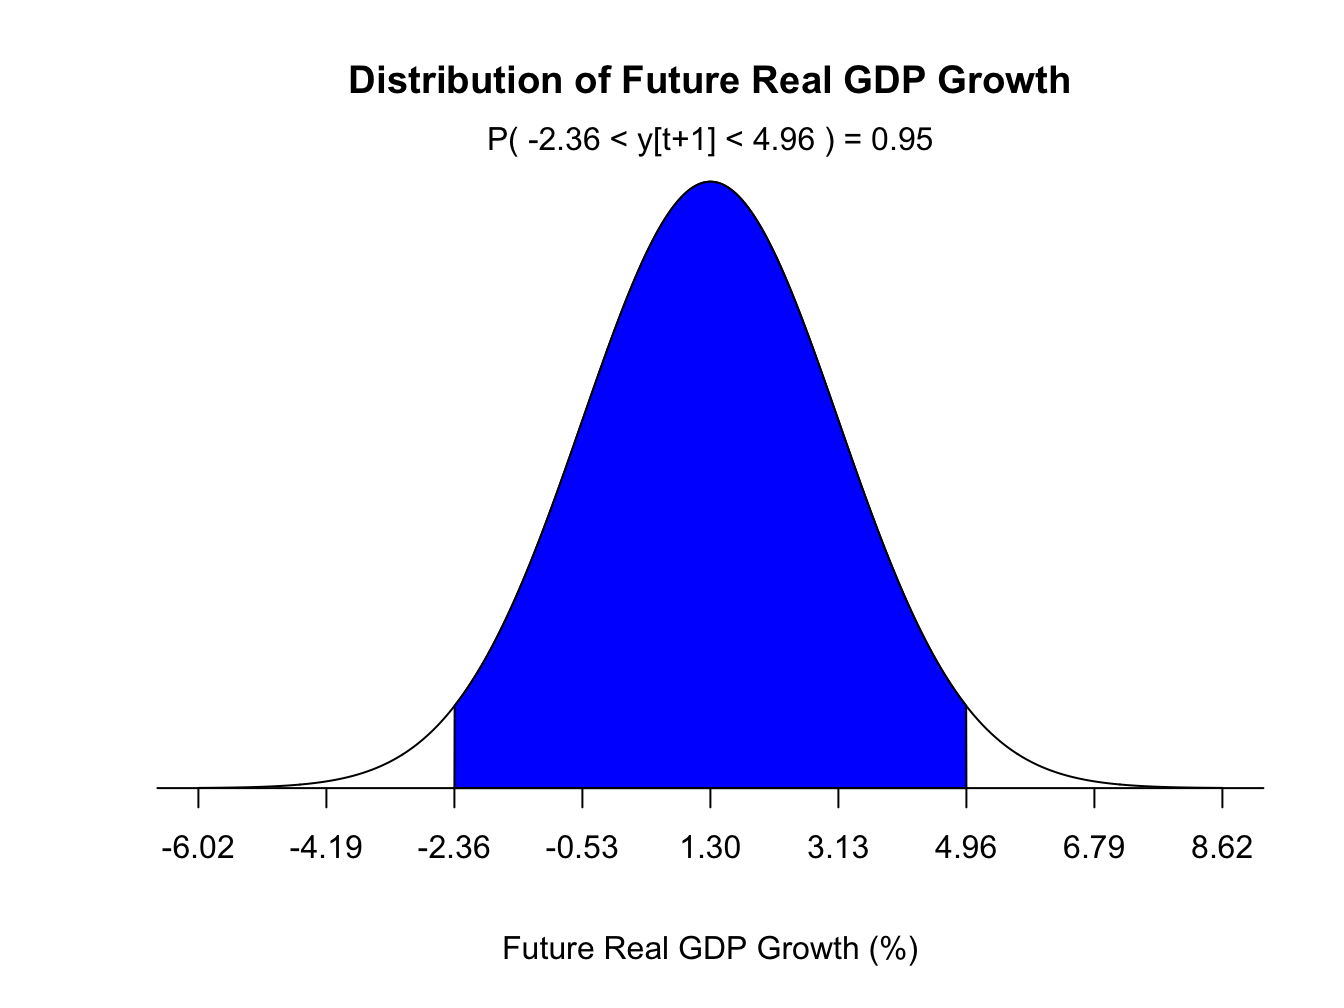
\includegraphics[width=0.8\linewidth]{bookdown-demo_files/figure-latex/figtwo-1} 

}

\caption{Density Forecast for Future Real GDP Growth}\label{fig:figtwo}
\end{figure}

\begin{enumerate}
\def\labelenumi{\arabic{enumi}.}
\setcounter{enumi}{1}
\tightlist
\item
  \emph{Point Forecast}: our forecast at each horizon is a single
  number. Often we use the expected value or mean as the point forecast.
  For example, the point forecast for the 1-period ahead real GDP growth
  can be the mean of the probability distribution of the future real GDP
  growth:

  \begin{equation}
  f_{t,1}=1.3%
  \end{equation}
\item
  \emph{Interval Forecast}: our forecast at each horizon is a range
  which is obtained by adding \emph{margin of errors} to the point
  forecast. With some probablity we expect our future value to fall
  withing this range. For example, the 95\% interval forecast for the
  next period real GDP growth is (-2.36\%,4.96\%). Hence, with 95\%
  confidence we expect next period GDP to fall between -2.36\% and
  4.96\%.
\end{enumerate}

\BeginKnitrBlock{definition}[Forecast Horizon]
\protect\hypertarget{def:d2}{}{\label{def:d2} \iffalse (Forecast Horizon)
\fi{} }
\EndKnitrBlock{definition} \emph{Forecast Horizon} is the number of
periods into the future for which we forecast a time series. We will
denote it by \(h\). Hence, for \(h=1\), we are looking at 1-period ahead
forecast, for \(h=2\) we are looking at 2-period ahead forecast and so
on.

Formally, for a given time series \(y_t\), the h-period ahead unknow
value is denoted by \(y_{t+h}\). The forecast of this value is denoted
\(f_{t,h}\).

\BeginKnitrBlock{definition}[Forecast Error]
\protect\hypertarget{def:d3}{}{\label{def:d3} \iffalse (Forecast Error)
\fi{} }
\EndKnitrBlock{definition}

A \emph{forecast error} is the difference between the realization of the
future value and the previously made forecast. Formally, the
\(h\)-period ahead forecast error is given by:

\begin{equation}
e_{t,h}=y_{t+h}-f_{t,h}
\end{equation}

Hence, for every horizon, we will have a forecast and a corresponding
forecast error. These errors can be negative (indicating over
prediction) or positive (indicating under prediction).

\BeginKnitrBlock{definition}[Information Set]
\protect\hypertarget{def:d4}{}{\label{def:d4} \iffalse (Information Set)
\fi{} }
\EndKnitrBlock{definition}

Forecasts are based on \emph{information} available at the time of
making the forecast. \emph{Information Set} contains all the relevant
information about the time series we would like to forecast. We denote
the set of information available at time \(T\) by \(\Omega_T\). There
are two types of information sets:

\begin{enumerate}
\def\labelenumi{\arabic{enumi}.}
\tightlist
\item
  Univariate Information set: Only includes hisorical data on the time
  series of interest:

  \begin{equation}
  \Omega_T=\{y_T, y_{T-1}, y_{T-2}, ...., y_1\}
  \end{equation}
\item
  Multivaiate Information set: Includes hisorical data on the time
  series of interest as well as any other variable(s) of interest. For
  example, suppose we have one more variable \(x\) that is relevant for
  forecasting \(y\). Then:

  \begin{equation}
  \Omega_T=\{y_T, x_T, y_{T-1}, x_{T-1}, y_{T-2},x_{T-2}. ...., y_1, x_1\}
  \end{equation}
\end{enumerate}

\section{Loss Function and Optimal
Forecast}\label{loss-function-and-optimal-forecast}

Think of a forecast as a solution to an \emph{optimization} problem.
When forecasts are wrong, the person making the forecast will suffer
some \emph{loss}. This loss will be a function of the magnitude as well
as the sign of the \emph{forecast error}. Hence, we can think of an
\emph{optimal forecast} as a solution to a minimization problem where
the forecaster is minimizing the loss from the forecast error.

\BeginKnitrBlock{definition}[Loss Function]
\protect\hypertarget{def:d5}{}{\label{def:d5} \iffalse (Loss Function) \fi{}
}
\EndKnitrBlock{definition}

A \emph{loss} function is a mapping between forecast errors and their
associated losses. Formally, we denote the h-period ahead loss function
by \(L(e_{t,h})\). For a function to be used as a loss function, three
properties must be satisfied:

\begin{enumerate}
\def\labelenumi{\arabic{enumi}.}
\tightlist
\item
  \(L(0)=0\)
\item
  \(\frac{dL}{de}>0\)
\item
  \(L(e)\) is a continuous function.
\end{enumerate}

Two types of loss functions are:

\begin{itemize}
\tightlist
\item
  Symmetric Loss Function: both positive and negative forecast errors
  lead to same loss. A commonly used loss function is \emph{quadratic
  loss function} given by:
\end{itemize}

\begin{equation}
L(e_{t,h})=e_{t,h}^2 = (y_{t+h}-f{t,h})^2
\end{equation}

\begin{itemize}
\tightlist
\item
  Asymmetric Loss Function: loss depends on the sign of the forecast
  error. For example, it could be that positive errors produce greater
  loss when compared to negative errors. See the function below that
  assumes a higher value for positive errors:
\end{itemize}

\begin{equation}
L(e_{t,h})=e_{t,h}^2+e_{t,h}
\end{equation}

Once we have chosen our loss function, the optimal forecast can be
obtained by minimizing the expected loss function.

\BeginKnitrBlock{definition}[Optimal Forecast]
\protect\hypertarget{def:d6}{}{\label{def:d6} \iffalse (Optimal Forecast)
\fi{} }
\EndKnitrBlock{definition}

An \emph{optimal forecast} minimizes the expected loss from the
forecast, given the information available at the time. Mathematically,
we denote it by \(f^*_{t,h}\) and it solves the following minimization
problem:

\begin{equation}
min_{f_{t,h}} E(L(e_{t,h})|\Omega_t)
\end{equation}

In theory we can assume any functional form for the loss function and
that will lead to a different \emph{optimal forecast}. An important
result that follows from a specific functional form is stated as Theorem
1.1.

\BeginKnitrBlock{theorem}
\protect\hypertarget{thm:unnamed-chunk-2}{}{\label{thm:unnamed-chunk-2} }If
the loss function is quadtratic then the optimal forecast is the
conditional mean of the time series of interest. Formally, if
\(L(e_{t,h})=e_{t,h}^2\) then,

\begin{equation}
f^*_{t,h}=E(y_{t+h}|\Omega_t)
\end{equation}
\EndKnitrBlock{theorem}

Note that \(E(e_{t,h}^2)\) is known as \emph{mean squared errors (MSE)}.
Hence, the expected loss from a quadratic loss function is the same as
the MSE. In this course, we assume that the forecaster faces a quadratic
loss function and hence based on Theorem 1.1, we will learn different
models for estimating the conditional mean of the future value of the
time series of interest, i.e., \(E(y_{t+h}|\Omega_t)\).

\chapter{Regression-based
Forecasting}\label{regression-based-forecasting}

One way to compute the conditional expectation is the linear regression
model. Here, our information set contains data on all relevant
explantory variacbles available at the time of forecast, i.e,

\begin{equation}
\Omega_t={X_{1t}, X_{2t},...X_{Kt}}
\end{equation}

Hence, we get the following equality:

\begin{equation}
E(y_t|\Omega_t)=E(y_{t+h}|X_{1t}, X_{2t}, X_{3t},...,X_{Kt})
\end{equation}

The right hand side of the above equation is the multiple regression
model of the form:

\begin{equation}
 y_{t}=\beta_0+\beta_1 X_{1t}+\beta_2 X_{2t}+..+\beta_K X_{Kt}+\epsilon_t
 \end{equation}

We can easily estimate the above model using Ordinary Least Squares
(OLS) and compute the \emph{predicted value} of \(y\):

\begin{equation}
    \widehat{y}_t = \widehat{\beta_0} +\widehat{\beta_1} X_{1t} +\widehat{\beta_2} X_{2t}+...+ \widehat{\beta_k} X_{Kt}
  \end{equation}

The above equation can be used to compute the optimal forecast. Suppose,
we are interested in computed the \(h\) period ahead forecast for \(y\).
Then, using the above equation we get:

\begin{equation}
        \widehat{y}_{t+h} =  \widehat{\beta_0} +\widehat{\beta_1} X_{1t+h} +\widehat{\beta_2} X_{2t+h}+...+ \widehat{\beta_k} X_{Kt+h}
    \end{equation}

\section{Scenario Analysis and Conditional
Forecasts}\label{scenario-analysis-and-conditional-forecasts}

One way to use a regression model to produce forecasts is called
\emph{scenario analysis} where we produce a different forecast for the
dependent under each possible scenario about the future values of the
independent variables. For example, what will be the forecast for
inflation if the Federal Reserve Bank raises the interest rate? Would
our forecast differ depending on the size of the increase in the
interest rate?

\section{Unconditional Forecasts}\label{unconditional-forecasts}

An alternative is to separately forecast each independent variable and
then compute the forecast for the dependent variable. Yet another
alternative is to use lagged variables as independent variables.
Depending on the number of lags, we can forecast that much ahead into
future (see Distributed Lag Section for details).

\section{Some practical issues}\label{some-practical-issues}

\begin{enumerate}
\def\labelenumi{\arabic{enumi}.}
\item
  To forecast the dependent variable we first need to compute a forecast
  for the independent variable. Errors in this step induce errors later.
\item
  \emph{Spurious regression}: It is quite possible to find a strong
  linear relationship between two completely unrelated variables over
  time if they share a common time trend.
\item
  \emph{Model Uncertainty}: We do not know the true functional form for
  the regression model and hence our estimated model is only a proxy for
  the true model.
\item
  \emph{Parameter Uncertainty}: This kind of forecast uses regression
  coefficients that are computed using a fixed sample. Over time with
  new data, there will be changes in these coefficients.
\end{enumerate}

\section{Distributed Lag Regression
Models}\label{distributed-lag-regression-models}

Consider the following simple regression model:

\begin{equation}
y_t= \beta_0 +\beta_1 x_t + \epsilon_t
\end{equation}

Here, if want to forecast \(y_{t+1}\) then we must either consider
different scenarios for \(x_{t+1}\) or indpendently forecast \(x_{t+1}\)
first, and then use it to compute forecast for \(y_{t+1}\). An
alternative is to estimate the following lagged regression model:

\begin{equation}
y_t= \beta_0 +\beta_1 x_{t-1} + \epsilon_t
\end{equation}

Note that by estimating the above model we get the following predicted
value equation for \(t+1\):

\begin{equation}
\widehat{y_{t+1}}=\widehat{\beta_0}+\widehat{\beta_1}x_{t}
\end{equation}

Hence, we can easily produce 1-period ahead forecast from this model. In
order to produce forecast farther into future we would need to add more
lags of the independent variable to the model. A generalized model of
this kind is called \emph{distributed lag model} and is given by:

\begin{equation}
y_t= \beta_0 +\sum_{s=1}^p\beta_s x_{t-s} + \epsilon_t
\end{equation}

The number of lags to include can be determined using some kind of
goodness of fit measure.

\section{Model Selection Criterion}\label{model-selection-criterion}

Most often we compare models that have different number of independent
variables. Here, we must account for the tradeoff between goodness of
fit and degrees of freedom. Increasing the number of independent
variables will:

\begin{enumerate}
\def\labelenumi{\arabic{enumi}.}
\item
  lower the MSE and hence leads to better fit.
\item
  lowers the degrees of freedom
\end{enumerate}

Two commonly used measures based on MSE incorporate this tradeoff:

\begin{enumerate}
\def\labelenumi{\arabic{enumi}.}
\tightlist
\item
  Akaike Information Criterion (AIC):
  \[ AIC= MSE \times e^{\frac{2k}{T}} \]
\end{enumerate}

where \(k\) is the number of estimated parameteris, \(T\) is the sample
size. Then, \(K/T\) is the number of parameters estimated per
observation and \(e^{\frac{2k}{T}}\) is the \emph{penalty factor}
imposed on adding more variables to the model. As we increase \(k\),
this penalty factor will increase exponentially for a giveb value of
\(T\).

\begin{enumerate}
\def\labelenumi{\arabic{enumi}.}
\setcounter{enumi}{1}
\tightlist
\item
  Bayesian Information Criterion (BIC):
\end{enumerate}

\[ BIC= MSE \times T^{\frac{k}{T}} \]

Lower values of either AIC or BIC indicates greater accuracy. So we
select a model with lower value of either of these two criteria. Note
that the penalty imposed by BIC is harsher and hence it will typically
select a more parsiomonius model.

\chapter{Components of a Time Series}\label{components-of-a-time-series}

A given time series can have four possible components:

\begin{enumerate}
\def\labelenumi{\arabic{enumi}.}
\item
  Trend: denoted by \(B_t\) captures the long run behavior of the time
  series of interest.
\item
  Season: denoted by \(S_t\) are \emph{periodic} fluctuations over
  \emph{seasons}. The period of the season is fixed and known. For
  example, rise in non-durable sales during Christmas.
\item
  Cycle: denoted by \(C_t\) are \emph{non-periodic} are flcutuations in
  that they occur regularly but over periods that are not fixed in
  duration.
\item
  Irregular: denoted by \(\epsilon_t\) are random fluctuations,
  typically modeled as a white noise process.
\end{enumerate}

\section{Decomposing a time series}\label{decomposing-a-time-series}

We can decompose any given time series into its components. There are
two ways to accomplish this:

\begin{enumerate}
\def\labelenumi{\arabic{enumi}.}
\tightlist
\item
  Additive Decomposition: Here it is assumed that all four components
  are added to obtain the underlying timer series:

  \begin{equation}
  y_t= B_t+S_t+C_t +\epsilon_t
  \end{equation}
\item
  Multiplicative Decomposition: Here it is assumed that all four
  components are multiplied to obtain the underlying timer series:

  \begin{equation}
  y_t= B_t \times S_t \times C_t \times \epsilon_t
  \end{equation}
\end{enumerate}

Note that using properties of logarithms, multiplicative decomposition
is the same as additive decomposition in log terms:

\begin{equation}
log(y_t)= log(B_t) + log(S_t) + log(C_t) + log(\epsilon_t)
\end{equation}

Most statistical softwares can implement these decompositions using data
on a time series variable as input. Typically they combine cyclical
component with irregular component and provide a three-way
decomposition. In Figure \ref{fig:figthree} I use R to decompose real
GDP for the US into its components.

\begin{figure}

{\centering 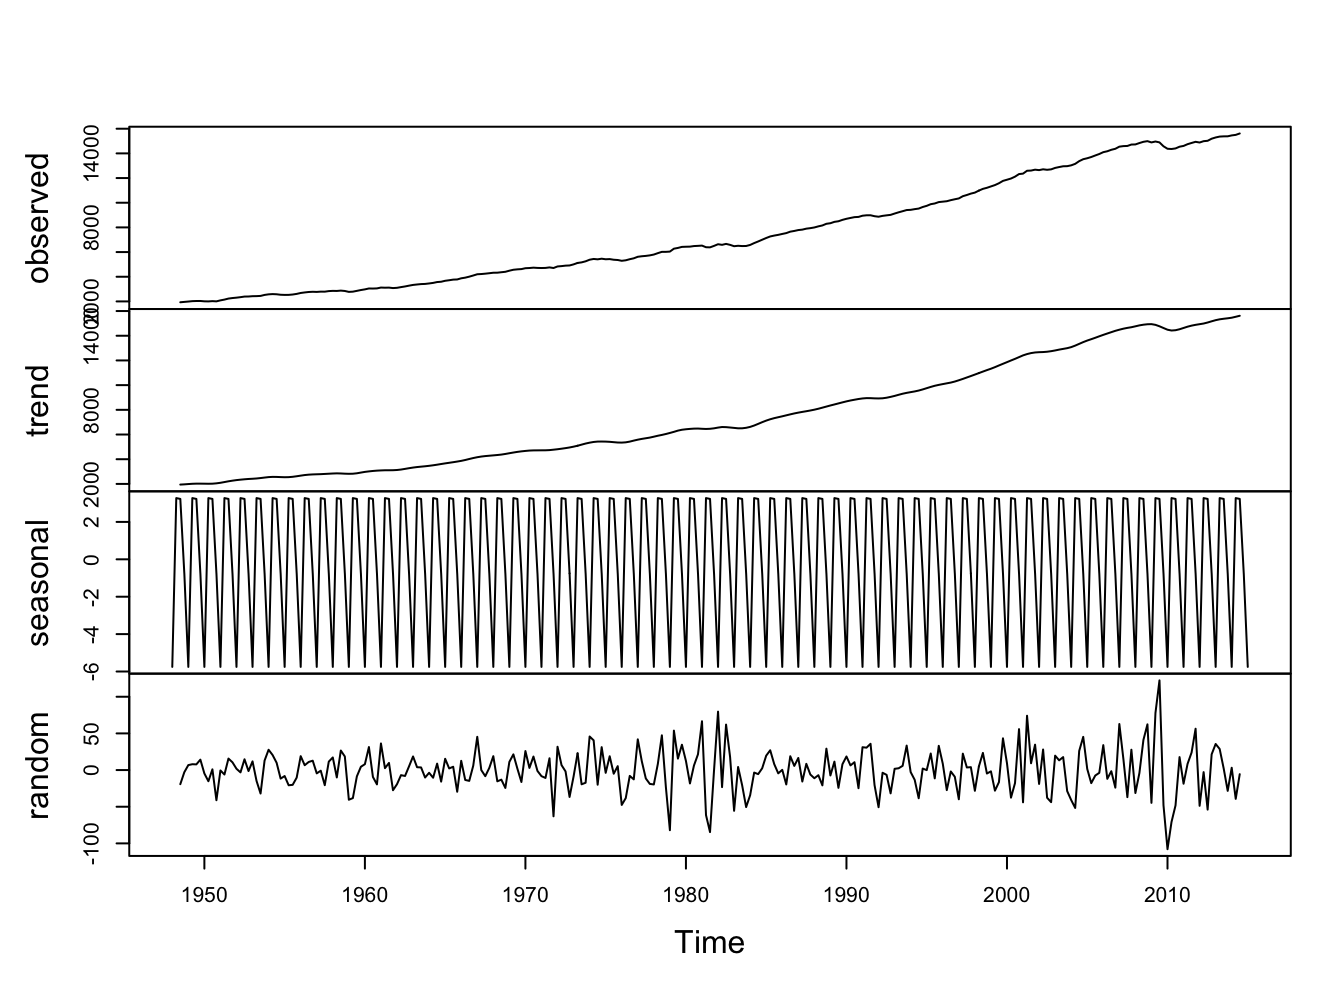
\includegraphics[width=0.8\linewidth]{bookdown-demo_files/figure-latex/figthree-1} 

}

\caption{ Additive Decomposition of Real GDP}\label{fig:figthree}
\end{figure}

\section{Uses of Decomposition of a time
series}\label{uses-of-decomposition-of-a-time-series}

The usefulness of decomposing a time series depends on our objective.

\begin{enumerate}
\def\labelenumi{\arabic{enumi}.}
\item
  It may be of interest to study each component separtaely or to simply
  improve our understanding of the temporal dynammics of a time series
  of interest. Decompositing it into different components is the first
  step towards achieving that goal.
\item
  We can also use the decomposition to filter out components that we are
  not interested in studying. If for example we are only interested in
  modeling the cyclical component of the time series, then we can assume
  some kind decomposition, additive or multiplicative, and filter out
  the trend and seasonal component. For example, assuming additive
  decomposition, the filtered time series is given by:

  \begin{equation}
  Filtered \ y_t= y_t-B_t-C_t
  \end{equation}
\end{enumerate}

We can then proceed to model the cyclical component using the filtered
data.

\chapter{Smoothing Methods}\label{smoothing-methods}

One way to approach forecasting is to \emph{average} out the
fluctuations in the underlying time series to produce a \emph{smoothed}
data which can be extrapolated to produce forecasts. These smoothing
methiods are essentially \emph{model-free} and may not even produce
\emph{optimal forecasts}. Depending on the method used one can
accomodate seasonal as well as trend components of the underlying time
series.

\section{Moving Average Method}\label{moving-average-method}

We compute an average of most recent data values for the time series and
use it as a forecast for the next period.

An important parameter is the \emph{window} over which we take the
average. Let us denote this window by \(m\), then:

\begin{equation}
    y^f_{T+1}=\frac{\sum_{i=t-m+1}^{t}{y_i}}{m}
    \end{equation}

A larger value of \(m\) produces greater smoothing and most softwares
have a default value of this parameter which can be changed if needed.

\section{Simple Exponential
Smoothing}\label{simple-exponential-smoothing}

In the moving average method, all obseravtions receieved same weight.
However, it is reasonable to argue that more recent observations may
have a greater influence than those in the remote past. In this methiod,
the weight attached to past observations exponentially decay over time.
Here is the algorthim for computing the smoothed data and its forecast:

\begin{enumerate}
\def\labelenumi{\arabic{enumi}.}
\item
  Initialize at t=1: \[y_1^s=y_1 \]
\item
  Update:
  \[      y_{t}^{s}= \alpha y_t + (1-\alpha)y_{t-1}^{s}  \quad for \ t=2,3,...T\]
\end{enumerate}

3: h-period ahead forecast:

\[  f_{T,h}= y_T^s\]

Here the h-period ahead forecast is:

\emph{Exercise: Can you show that \(y_{t}^{s}\) is a is the weighted
moving average of all past observations? Use backward substitution
method.}

Here \(\alpha \in (0,1)\) is the smoothing parameter, with smaller value
indicating greater smoothing.

\section{Holt-Winters Smoothing}\label{holt-winters-smoothing}

We add trend component to the simple exponential smoothing. In step 2
the equation we use to update the smoothed data is given by:

\begin{equation}
    y_{t}^{s}= \alpha y_t + (1-\alpha)(y_{t-1}^{s}+B_{t-1})\\
    B_t = \beta (y_t^s -y_{t-1}^s) + (1-\beta) B_{t-1}
 \end{equation}

We now have an additional parameter \(\beta\) that is the trend
parameter. Here the h-period ahead forecast is:

\begin{equation}
  f_{T,h} = y_T^s + h\times B_T
  \end{equation}

\section{Holt-Winters Smoothing with
Seasonality}\label{holt-winters-smoothing-with-seasonality}

We now add seasonal component along with trend. Assuming multiplicative
seasonality with period \(n\):

\begin{equation}
    y_{t}^{s}= \alpha \frac{y_t}{S_{t-n}} + (1-\alpha)(y_{t-1}^{s}+B_{t-1})\\
    B_t = \gamma (y_t^s -y_{t-1}^s) + (1-\gamma) B_{t-1}\\
    S_t = \beta\frac{y_t}{y_t^s}+(1-\beta)S_{t-n}
  \end{equation}

The h-period ahead forecast is given by:

\begin{equation}
    f_{T,h}= (y_T^s + h\times B_T) \times S_{T+h-n}
   \end{equation}

\section{Application}\label{application}

We use R to implement a 12-period ahead forecast for retail sales for
the U.S. The data is at monthly frequency from 1959 through 2015. We use
natural logs of the data and compute smoothed series using each of the
three methods. The resulting forecasts are ploted in Figure
\ref{fig:figfour}.

\begin{figure}

{\centering 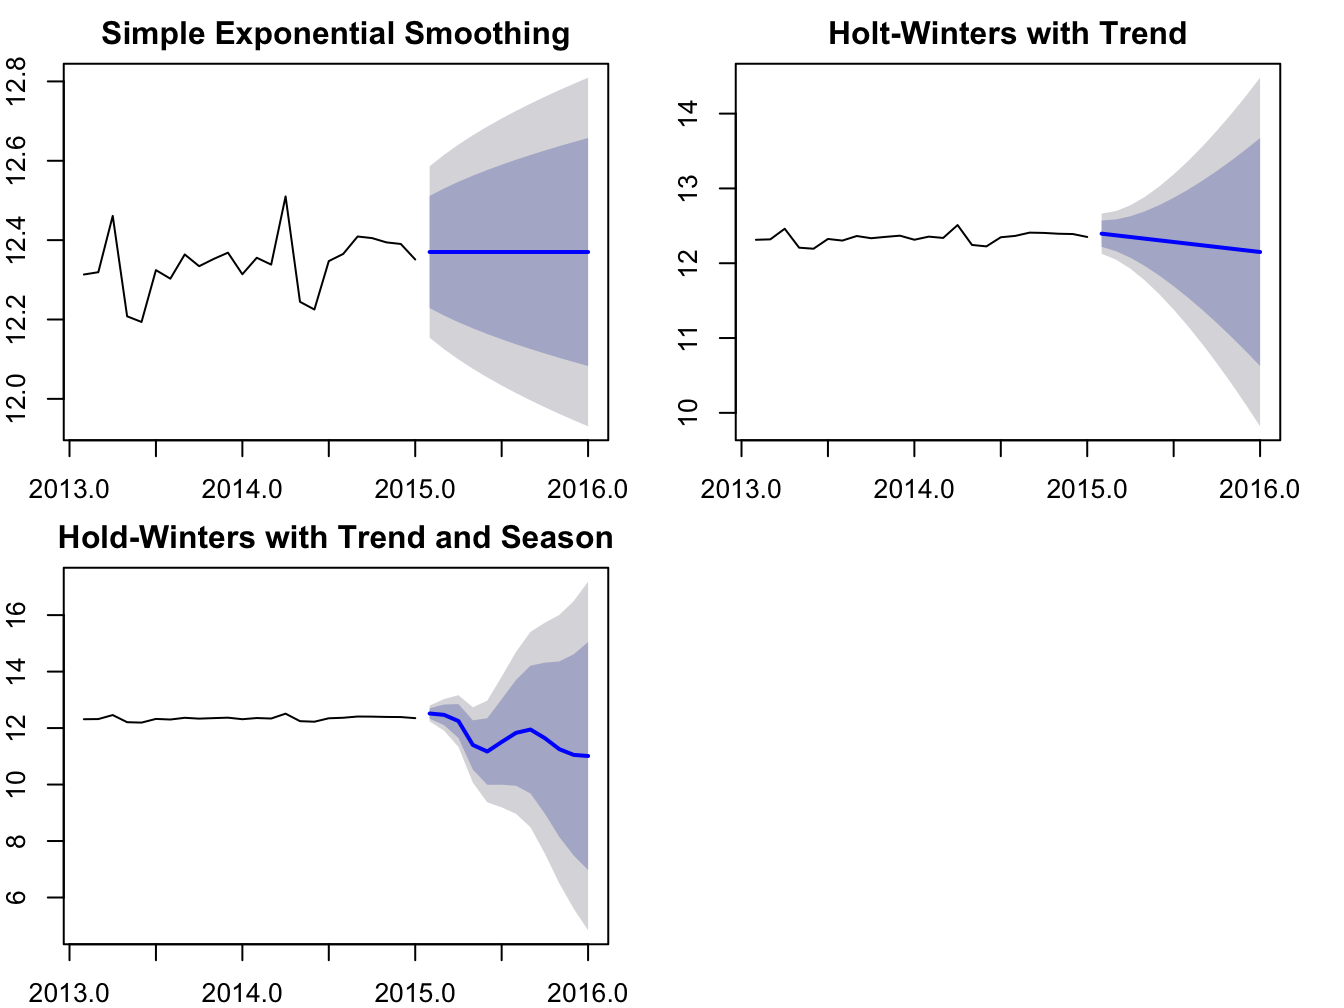
\includegraphics[width=0.8\linewidth]{bookdown-demo_files/figure-latex/figfour-1} 

}

\caption{Forecast of Retail Sales: Three Smoothing Methods}\label{fig:figfour}
\end{figure}

\chapter{Autoregressive Moving Average
(ARIMA)}\label{autoregressive-moving-average-arima}

\section{Covariance Stationary Time
Series}\label{covariance-stationary-time-series}

\BeginKnitrBlock{definition}[Covariance Stationary Time Series]
\protect\hypertarget{def:d1}{}{\label{def:d1} \iffalse (Covariance
Stationary Time Series) \fi{} }
\EndKnitrBlock{definition} A time series \(\{y_t\}\) is said to be a
\emph{covariance stationary process} if:

\begin{enumerate}
\def\labelenumi{\arabic{enumi}.}
\tightlist
\item
  \(E(y_t)=\mu_x \quad \forall \quad t\)
\item
  \(Var(y_t)=\sigma_x^2 \quad \forall \quad t\)
\item
  \(Cov(y_t,y_{t-s})=\gamma(s) \quad \forall \quad s\neq t\)
\end{enumerate}

\section{Correlation over time}\label{correlation-over-time}

In general, for a time series, \(\{y_t\}\),

\begin{align}
    Cor(y_t,y_{t-s})=\frac{ Cov(y_t,y_{t-s})}{\sqrt{\sigma^2_{y_t} \times \sigma^2_{y_{t-s}}}}
        \end{align}

where \(Cov(y_t,y_{t-s})= E(y_t-\mu_{y_t})(y_{t-s}-\mu_{y_{t-s}})\) and
\(\sigma^2_{y_t}=E(y_t-\mu_{y_t})^2\)

\BeginKnitrBlock{definition}[Auto Correlation Function (ACF)]
\protect\hypertarget{def:d2}{}{\label{def:d2} \iffalse (Auto Correlation
Function (ACF)) \fi{} }
\EndKnitrBlock{definition}

An \emph{ACF} plots the correlation of a time series with its own past
values over time. For a stationary time series, using the three
conditions we get:

\begin{align}
    ACF(s) \ or \ \rho(s)=\frac{\gamma(s)}{\gamma(0)}
    \end{align}

\BeginKnitrBlock{definition}[Partial Auto Correlation Function (PACF)]
\protect\hypertarget{def:d3}{}{\label{def:d3} \iffalse (Partial Auto
Correlation Function (PACF)) \fi{} }
\EndKnitrBlock{definition} The \emph{partial autocorrelation function
(PACF)} for a stationary time series \(y_t\) at lag \(s\) is the direct
correlation between \(y_t\) and \(y_{t-s}\), after filtering out the
linear influence of \$ y\_\{t-1\},\ldots,y\_\{t-s-1\}\$ on \(y_t\).

\section{Autoregressive (AR) Model}\label{autoregressive-ar-model}

A \emph{stationary}time series \(\{x_t\}\) can be modeled as an AR(p)
process:

\begin{equation}
 y_t = \phi_0 +\phi_1 y_{t-1} + \phi_2 y_{t-2} + ...... + \phi_p y_{t-p}+\epsilon_t
 \end{equation}

\section{Moving Average (MA) Model}\label{moving-average-ma-model}

A \emph{stationary} time series \(\{y_t\}\) can be modeled as an MA(q)
process:

\begin{equation}
  y_t = \theta_0 + \epsilon_t + \theta_1 \epsilon_{t-1} + \theta_2 \epsilon_{t-2} + ...... + \theta_q \epsilon_{t-q}
    \end{equation}

\section{ARMA(p, q)\}}\label{armap-q}

An ARMA model simply combines both AR and MA components to model the
dynamics of a time series. Formula,

\begin{equation}
   y_t = \phi_0 +\phi_1 x_{t-1} + \phi_2 y_{t-2} + ...... + \phi_p y_{t-p}+\epsilon_t + \theta_1 \epsilon_{t-1} + \theta_2 \epsilon_{t-2} + ...... + \theta_q \epsilon_{t-q}
   \end{equation}

\chapter{Modeling Volatility}\label{modeling-volatility}

\chapter{Vector Autoregresson (VAR)}\label{vector-autoregresson-var}

\bibliography{book.bib,packages.bib}


\end{document}
